% Options for packages loaded elsewhere
\PassOptionsToPackage{unicode}{hyperref}
\PassOptionsToPackage{hyphens}{url}
\PassOptionsToPackage{dvipsnames,svgnames,x11names}{xcolor}
%
\documentclass[
  ignorenonframetext,
]{beamer}
\usepackage{pgfpages}
\setbeamertemplate{caption}[numbered]
\setbeamertemplate{caption label separator}{: }
\setbeamercolor{caption name}{fg=normal text.fg}
\beamertemplatenavigationsymbolsempty
% Prevent slide breaks in the middle of a paragraph
\widowpenalties 1 10000
\raggedbottom

\usepackage{amsmath,amssymb}
\usepackage{iftex}
\ifPDFTeX
  \usepackage[T1]{fontenc}
  \usepackage[utf8]{inputenc}
  \usepackage{textcomp} % provide euro and other symbols
\else % if luatex or xetex
  \usepackage{unicode-math}
  \defaultfontfeatures{Scale=MatchLowercase}
  \defaultfontfeatures[\rmfamily]{Ligatures=TeX,Scale=1}
\fi
\usepackage{lmodern}
\usetheme[]{AnnArbor}
\usecolortheme{dolphin}
\usefonttheme{structurebold}
\ifPDFTeX\else  
    % xetex/luatex font selection
\fi
% Use upquote if available, for straight quotes in verbatim environments
\IfFileExists{upquote.sty}{\usepackage{upquote}}{}
\IfFileExists{microtype.sty}{% use microtype if available
  \usepackage[]{microtype}
  \UseMicrotypeSet[protrusion]{basicmath} % disable protrusion for tt fonts
}{}
\makeatletter
\@ifundefined{KOMAClassName}{% if non-KOMA class
  \IfFileExists{parskip.sty}{%
    \usepackage{parskip}
  }{% else
    \setlength{\parindent}{0pt}
    \setlength{\parskip}{6pt plus 2pt minus 1pt}}
}{% if KOMA class
  \KOMAoptions{parskip=half}}
\makeatother
\usepackage{xcolor}
\newif\ifbibliography
\setlength{\emergencystretch}{3em} % prevent overfull lines
\setcounter{secnumdepth}{-\maxdimen} % remove section numbering


\providecommand{\tightlist}{%
  \setlength{\itemsep}{0pt}\setlength{\parskip}{0pt}}\usepackage{longtable,booktabs,array}
\usepackage{calc} % for calculating minipage widths
\usepackage{caption}
% Make caption package work with longtable
\makeatletter
\def\fnum@table{\tablename~\thetable}
\makeatother
\usepackage{graphicx}
\makeatletter
\def\maxwidth{\ifdim\Gin@nat@width>\linewidth\linewidth\else\Gin@nat@width\fi}
\def\maxheight{\ifdim\Gin@nat@height>\textheight\textheight\else\Gin@nat@height\fi}
\makeatother
% Scale images if necessary, so that they will not overflow the page
% margins by default, and it is still possible to overwrite the defaults
% using explicit options in \includegraphics[width, height, ...]{}
\setkeys{Gin}{width=\maxwidth,height=\maxheight,keepaspectratio}
% Set default figure placement to htbp
\makeatletter
\def\fps@figure{htbp}
\makeatother
% definitions for citeproc citations
\NewDocumentCommand\citeproctext{}{}
\NewDocumentCommand\citeproc{mm}{%
  \begingroup\def\citeproctext{#2}\cite{#1}\endgroup}
\makeatletter
 % allow citations to break across lines
 \let\@cite@ofmt\@firstofone
 % avoid brackets around text for \cite:
 \def\@biblabel#1{}
 \def\@cite#1#2{{#1\if@tempswa , #2\fi}}
\makeatother
\newlength{\cslhangindent}
\setlength{\cslhangindent}{1.5em}
\newlength{\csllabelwidth}
\setlength{\csllabelwidth}{3em}
\newenvironment{CSLReferences}[2] % #1 hanging-indent, #2 entry-spacing
 {\begin{list}{}{%
  \setlength{\itemindent}{0pt}
  \setlength{\leftmargin}{0pt}
  \setlength{\parsep}{0pt}
  % turn on hanging indent if param 1 is 1
  \ifodd #1
   \setlength{\leftmargin}{\cslhangindent}
   \setlength{\itemindent}{-1\cslhangindent}
  \fi
  % set entry spacing
  \setlength{\itemsep}{#2\baselineskip}}}
 {\end{list}}
\usepackage{calc}
\newcommand{\CSLBlock}[1]{\hfill\break\parbox[t]{\linewidth}{\strut\ignorespaces#1\strut}}
\newcommand{\CSLLeftMargin}[1]{\parbox[t]{\csllabelwidth}{\strut#1\strut}}
\newcommand{\CSLRightInline}[1]{\parbox[t]{\linewidth - \csllabelwidth}{\strut#1\strut}}
\newcommand{\CSLIndent}[1]{\hspace{\cslhangindent}#1}


% logo
\titlegraphic{
\includegraphics[width=4cm]{000_logos/logo-blue-vertical}}
\logo{\ifnum\thepage>1
\includegraphics[width=0.5cm]{000_logos/logo-blue-vertical}\fi}

% UMNG: Manual de image institucional

% Colors

% Umng
\definecolor{yellow}{HTML}{fdc600}
\definecolor{red}{HTML}{ee2a24}

% Estudios a Distancia
\definecolor{blue1}{HTML}{12245b}
\definecolor{blue2}{HTML}{767ca6}
\definecolor{blue3}{HTML}{cad2ec}

% Modify items
\setbeamercolor{palette primary}{bg=blue3}
\setbeamercolor{palette tertiary}{bg=blue1}
\setbeamercolor{frametitle}{bg=yellow}

% Hyperlinks
\hypersetup{
  linkcolor=red,
  citecolor=red
}

\makeatletter
\@ifpackageloaded{caption}{}{\usepackage{caption}}
\AtBeginDocument{%
\ifdefined\contentsname
  \renewcommand*\contentsname{Table of contents}
\else
  \newcommand\contentsname{Table of contents}
\fi
\ifdefined\listfigurename
  \renewcommand*\listfigurename{List of Figures}
\else
  \newcommand\listfigurename{List of Figures}
\fi
\ifdefined\listtablename
  \renewcommand*\listtablename{List of Tables}
\else
  \newcommand\listtablename{List of Tables}
\fi
\ifdefined\figurename
  \renewcommand*\figurename{Figure}
\else
  \newcommand\figurename{Figure}
\fi
\ifdefined\tablename
  \renewcommand*\tablename{Table}
\else
  \newcommand\tablename{Table}
\fi
}
\@ifpackageloaded{float}{}{\usepackage{float}}
\floatstyle{ruled}
\@ifundefined{c@chapter}{\newfloat{codelisting}{h}{lop}}{\newfloat{codelisting}{h}{lop}[chapter]}
\floatname{codelisting}{Listing}
\newcommand*\listoflistings{\listof{codelisting}{List of Listings}}
\makeatother
\makeatletter
\makeatother
\makeatletter
\@ifpackageloaded{caption}{}{\usepackage{caption}}
\@ifpackageloaded{subcaption}{}{\usepackage{subcaption}}
\makeatother

\ifLuaTeX
\usepackage[bidi=basic]{babel}
\else
\usepackage[bidi=default]{babel}
\fi
\babelprovide[main,import]{english}
% get rid of language-specific shorthands (see #6817):
\let\LanguageShortHands\languageshorthands
\def\languageshorthands#1{}
\ifLuaTeX
  \usepackage{selnolig}  % disable illegal ligatures
\fi
\usepackage{bookmark}

\IfFileExists{xurl.sty}{\usepackage{xurl}}{} % add URL line breaks if available
\urlstyle{same} % disable monospaced font for URLs
\hypersetup{
  pdftitle={Strategy and Tactics of Distributive Bargaining},
  pdfauthor={Luis Francisco Gómez López},
  pdflang={en},
  colorlinks=true,
  linkcolor={Maroon},
  filecolor={Maroon},
  citecolor={Blue},
  urlcolor={Blue},
  pdfcreator={LaTeX via pandoc}}


\title{Strategy and Tactics of Distributive Bargaining}
\author{Luis Francisco Gómez López}
\date{2024-07-22}
\institute{FAEDIS}

\begin{document}
\frame{\titlepage}

\renewcommand*\contentsname{Table of contents}
\begin{frame}[allowframebreaks]
  \frametitle{Table of contents}
  \tableofcontents[hideallsubsections]
\end{frame}

\section{Please Read Me}\label{please-read-me}

\begin{frame}{}
\phantomsection\label{section}
\begin{itemize}
\item
  Check the message \textbf{Welcome greeting} published in the News
  Bulletin Board.
\item
  Dear student please edit your profile uploading a photo where your
  face is clearly visible.
\item
  The purpose of the virtual meetings is to answer questions and not to
  make a summary of the study material.
\item
  This presentation is based on
  (\citeproc{ref-lewicki_negociacion_2024}{Lewicki, Barry, and Saunders
  2024, chap. 2})
\end{itemize}
\end{frame}

\section{Purpose}\label{purpose}

\begin{frame}{}
\phantomsection\label{section-1}
Understand the basic elements of a distributive negotiation situation,
as well as the strategies and tactics that can be applied in this
context.
\end{frame}

\section{Elements of a distributive negotiation
situation}\label{elements-of-a-distributive-negotiation-situation}

\begin{frame}{}
\phantomsection\label{section-2}
\definecolor{red}{RGB}{227, 26, 28}
\definecolor{blue}{RGB}{44, 62, 80}

\begin{itemize}
\item
  Buyer: Jackson (\(\color{blue}{J}\)) and Seller: Sofia
  (\(\color{red}{S}\))\footnote<.->{Both \(\color{blue}{J}\) and
    \(\color{red}{S}\) have a common interest in cooperating but
    conflicting interests on how exactly to cooperate. For that reason a
    negotiation situation arises
    (\citeproc{ref-muthoo_bargaining_1999}{Muthoo 1999})}

  \begin{itemize}
  \tightlist
  \item
    Resistance point \(\color{blue}{J}\), \(\color{blue}{Rp_J}\): 150K
    USD
  \item
    Resistance point \(\color{red}{S}\), \(\color{red}{Rp_S}\): 130K USD
  \end{itemize}
\end{itemize}

\begin{figure}

\centering{

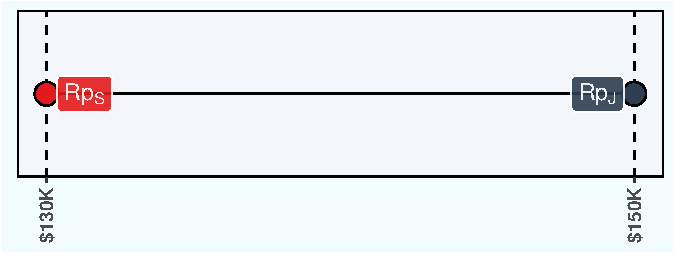
\includegraphics[width=0.85\textwidth,height=\textheight]{002_stra_tac_distri_files/figure-beamer/fig-resistance-point-1.pdf}

}

\caption{\label{fig-resistance-point}Resistance points}

\end{figure}%
\end{frame}

\begin{frame}{}
\phantomsection\label{section-3}
\definecolor{red}{RGB}{227, 26, 28}
\definecolor{blue}{RGB}{44, 62, 80}

\begin{itemize}
\item
  Buyer: Jackson (\(\color{blue}{J}\)) and Seller: Sofia
  (\(\color{red}{S}\))

  \begin{itemize}
  \tightlist
  \item
    Initial offer \(\color{blue}{J}\), \(\color{blue}{Io_J}\): 133K USD
  \item
    Initial offer \(\color{red}{S}\), \(\color{red}{Io_S}\): 145K USD
  \end{itemize}
\end{itemize}

\begin{figure}

\centering{

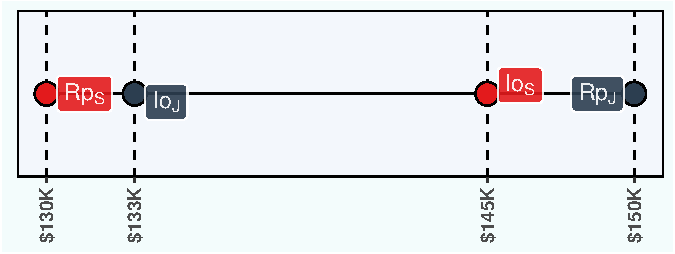
\includegraphics[width=0.85\textwidth,height=\textheight]{002_stra_tac_distri_files/figure-beamer/fig-initial-offer-1.pdf}

}

\caption{\label{fig-initial-offer}Initial offers}

\end{figure}%
\end{frame}

\begin{frame}{}
\phantomsection\label{section-4}
\definecolor{red}{RGB}{227, 26, 28}
\definecolor{blue}{RGB}{44, 62, 80}

\begin{itemize}
\item
  Buyer: Jackson (\(\color{blue}{J}\)) and Seller: Sofia
  (\(\color{red}{S}\))

  \begin{itemize}
  \tightlist
  \item
    Target point \(\color{blue}{J}\), \(\color{blue}{Tp_J}\): 135K USD
  \item
    Target point \(\color{red}{S}\), \(\color{red}{Tp_S}\): 140K USD
  \end{itemize}
\end{itemize}

\begin{figure}

\centering{

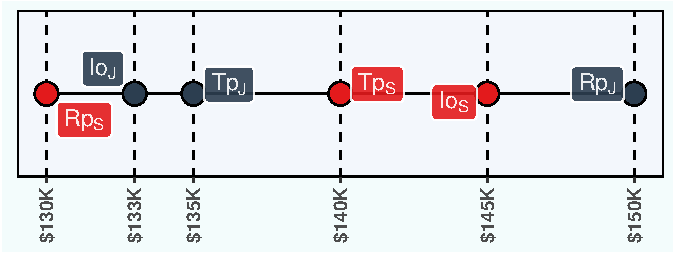
\includegraphics[width=0.85\textwidth,height=\textheight]{002_stra_tac_distri_files/figure-beamer/fig-target-point-1.pdf}

}

\caption{\label{fig-target-point}Target points}

\end{figure}%
\end{frame}

\begin{frame}{}
\phantomsection\label{section-5}
\definecolor{red}{RGB}{227, 26, 28}
\definecolor{blue}{RGB}{44, 62, 80}

\begin{itemize}
\item
  Buyer: Jackson (\(\color{blue}{J}\)) and Seller: Sofia
  (\(\color{red}{S}\))

  \begin{itemize}
  \tightlist
  \item
    BATNA \(\color{blue}{J}\), \(\color{blue}{BATNA_J}\): 142K USD
  \item
    BATNA \(\color{red}{S}\), \(\color{red}{BATNA_S}\): 134K USD
  \end{itemize}
\end{itemize}

\begin{figure}

\centering{

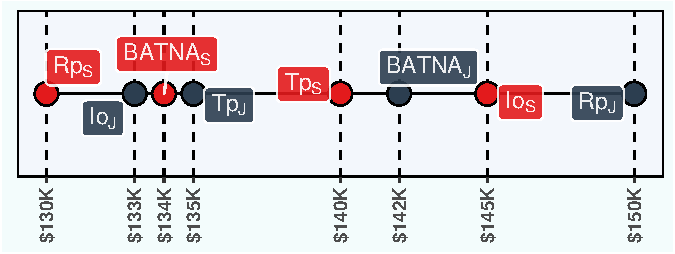
\includegraphics[width=0.85\textwidth,height=\textheight]{002_stra_tac_distri_files/figure-beamer/fig-batna-1.pdf}

}

\caption{\label{fig-batna}Best alternatives to a negotiated agreement}

\end{figure}%
\end{frame}

\begin{frame}{}
\phantomsection\label{section-6}
\definecolor{red}{RGB}{227, 26, 28}
\definecolor{blue}{RGB}{44, 62, 80}

\begin{itemize}
\item
  Buyer: Jackson (\(\color{blue}{J}\)) and Seller: Sofia
  (\(\color{red}{S}\))

  \begin{itemize}
  \item
    Bargaining range\footnote<.->{Also known as settlement range or zone
      of potential agreement}: \([\text{\$130K},\text{\$150K}]\)

    \begin{itemize}
    \tightlist
    \item
      Is the result of
      \([\text{\$130K}, \infty) \cap [0, \text{\$150K}]\)
    \item
      If the bargaining range is \(\neq \emptyset\),
      \(Rp_S \leq BATNA_J\) and \(BATNA_S \leq Rp_J\) then an aggrement
      between \(\color{blue}{J}\) and \(\color{red}{S}\) is possible
    \end{itemize}
  \end{itemize}
\end{itemize}

\begin{figure}

\centering{

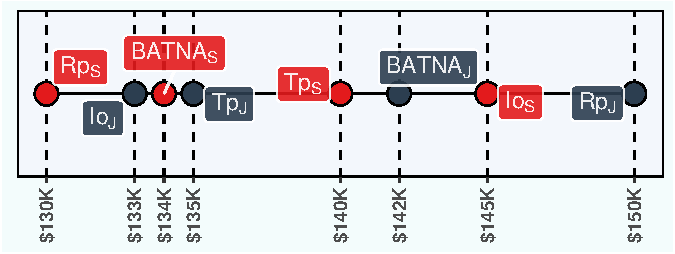
\includegraphics[width=0.85\textwidth,height=\textheight]{002_stra_tac_distri_files/figure-beamer/fig-bargaining-range-1.pdf}

}

\caption{\label{fig-bargaining-range}Bargaining range}

\end{figure}%
\end{frame}

\begin{frame}{}
\phantomsection\label{section-7}
\definecolor{red}{RGB}{227, 26, 28}
\definecolor{blue}{RGB}{44, 62, 80}

\begin{itemize}
\item
  Buyer: Jackson (\(\color{blue}{J}\)) and Seller: Sofia
  (\(\color{red}{S}\))

  \begin{itemize}
  \tightlist
  \item
    In this example the settlement point
    \(\in [Tp_J, Tp_S] = [\text{\$135K}, \text{\$140K}]\)
  \end{itemize}
\end{itemize}

\begin{figure}

\centering{

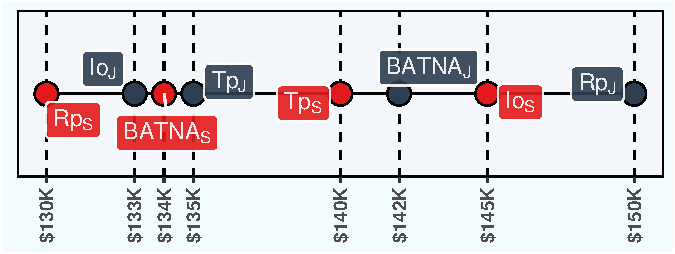
\includegraphics[width=0.85\textwidth,height=\textheight]{002_stra_tac_distri_files/figure-beamer/fig-settlement-point-1.pdf}

}

\caption{\label{fig-settlement-point}Possible values for a settlement
point}

\end{figure}%
\end{frame}

\begin{frame}{}
\phantomsection\label{section-8}
\definecolor{red}{RGB}{227, 26, 28}
\definecolor{blue}{RGB}{44, 62, 80}

\begin{itemize}
\item
  In the case of a distributive negotiation, it is most likely that the
  settlement point does not correspond to the target points of the
  participants in the negotiation.
\item
  In the example of \(\color{blue}{J}\) and \(\color{red}{S}\) it was
  implicitly assumed that the negotiation element was the price. This
  element is known as a \textbf{bargaining mix}\footnote<.->{It is
    define as the set of issues that will be negotiated} where it does
  not necessarily have to be a single element.

  \begin{itemize}
  \tightlist
  \item
    For example \(\color{blue}{J}\) and \(\color{red}{S}\) also can
    include in the bargaining mix the final date of the sale, whether or
    not renovations are included or if other items such as furniture and
    household appliances are added.
  \end{itemize}
\end{itemize}
\end{frame}

\section{Strategies}\label{strategies}

\begin{frame}{}
\phantomsection\label{section-9}
\begin{figure}

\centering{

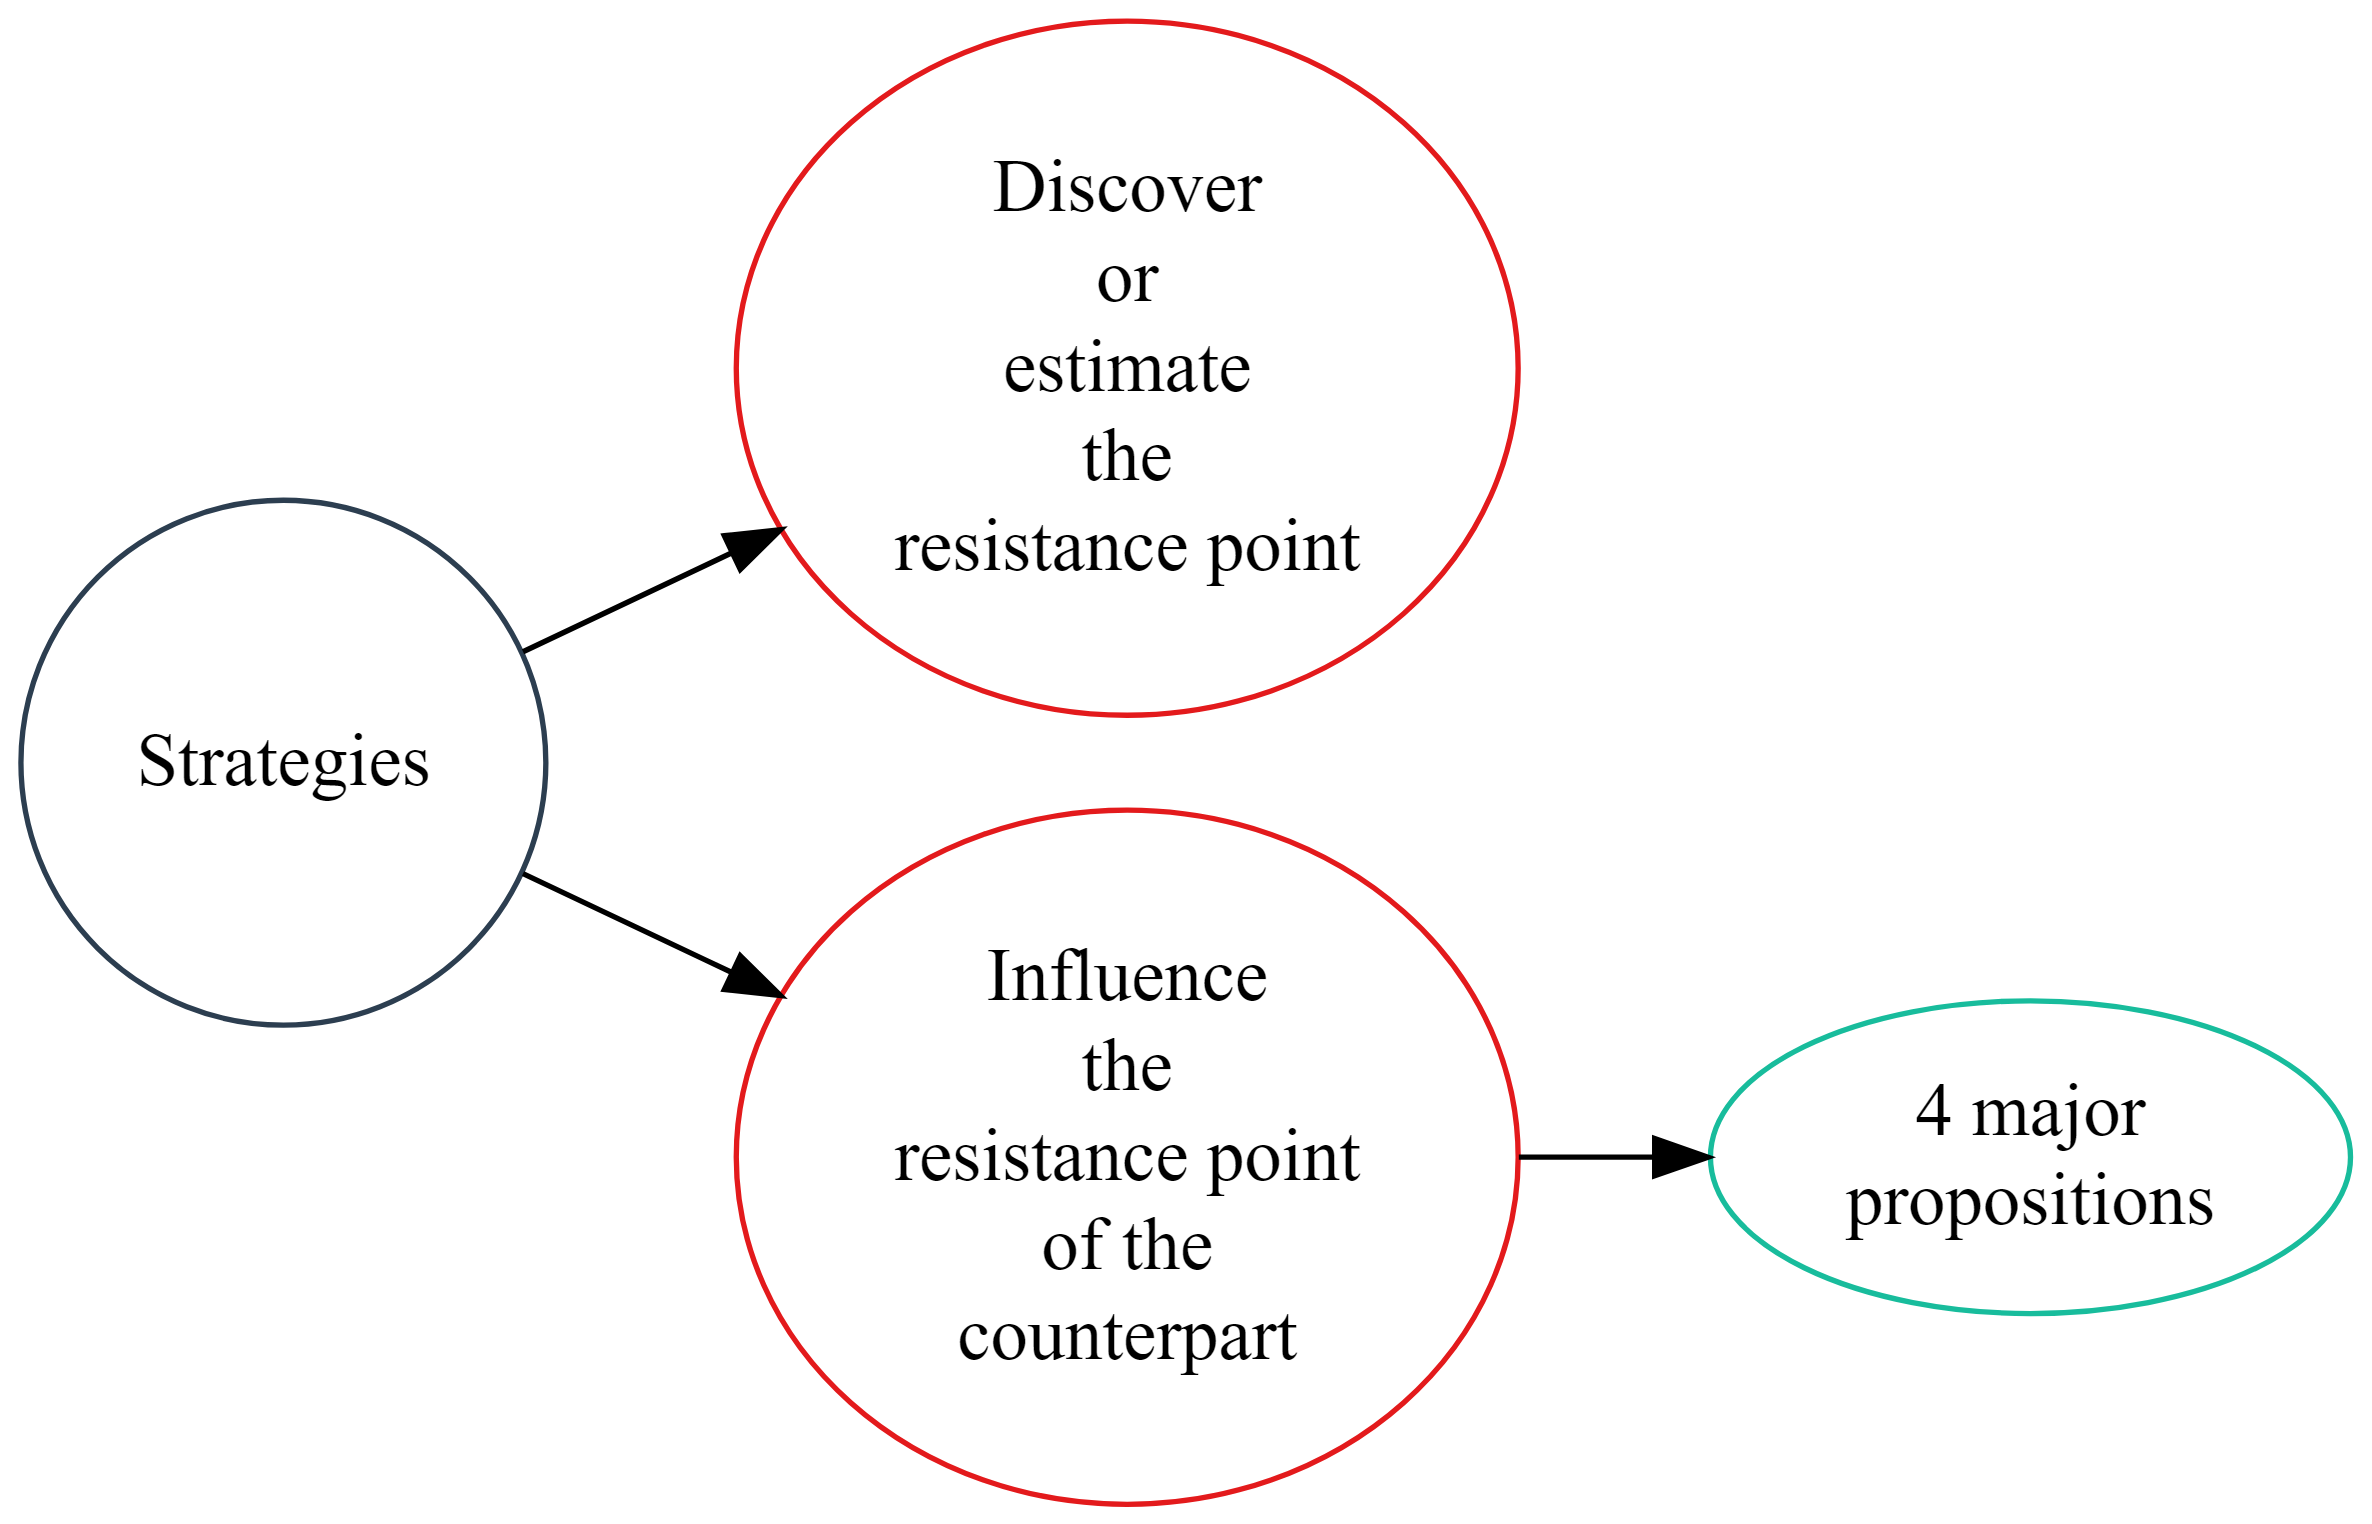
\includegraphics[width=5.5in,height=2.5in]{002_stra_tac_distri_files/figure-beamer/dot-figure-1.png}

}

\caption{\label{fig-strategies-distributive-bargaining}Strategies
distributive bargaining
(\citeproc{ref-lewicki_negociacion_2024}{Lewicki, Barry, and Saunders
2024, 39--41})}

\end{figure}%
\end{frame}

\section{Tactics}\label{tactics}

\begin{frame}{}
\phantomsection\label{section-10}
\begin{figure}

\centering{

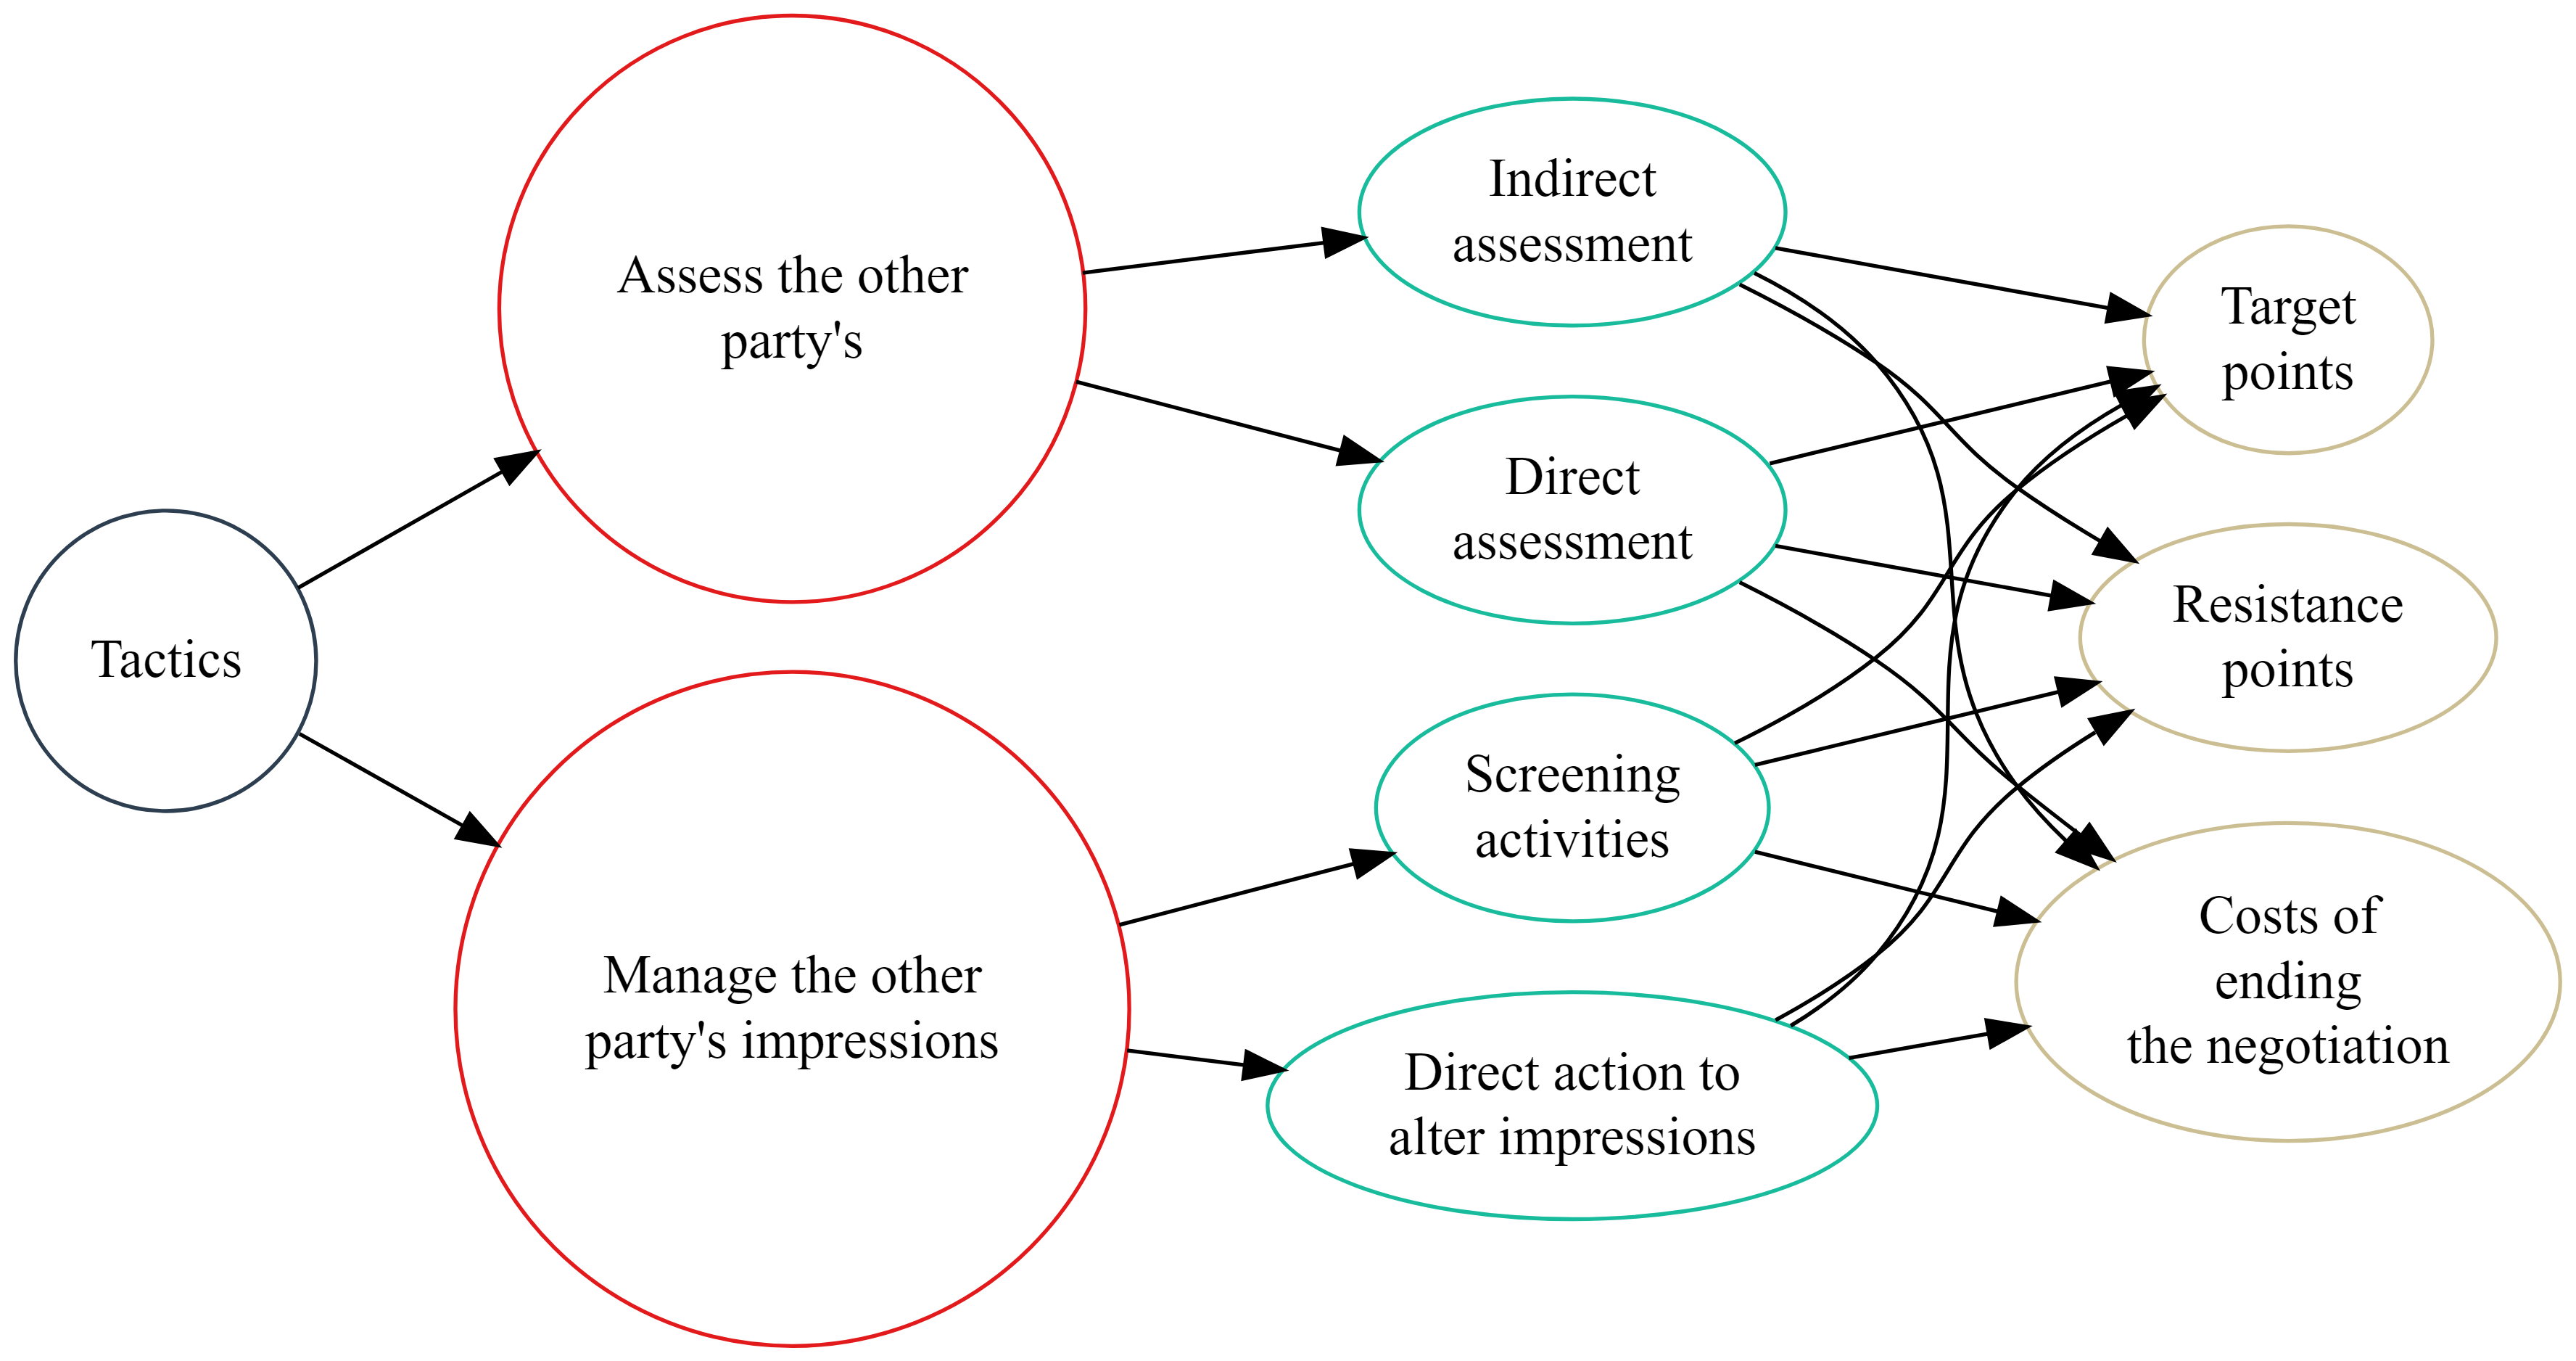
\includegraphics[width=4.5in,height=2.5in]{002_stra_tac_distri_files/figure-beamer/dot-figure-5.png}

}

\caption{\label{fig-tactics-distributive-bargaining-1}Tactics
distributive bargaining
(\citeproc{ref-lewicki_negociacion_2024}{Lewicki, Barry, and Saunders
2024, 42--48})}

\end{figure}%
\end{frame}

\begin{frame}{}
\phantomsection\label{section-11}
\begin{figure}

\centering{

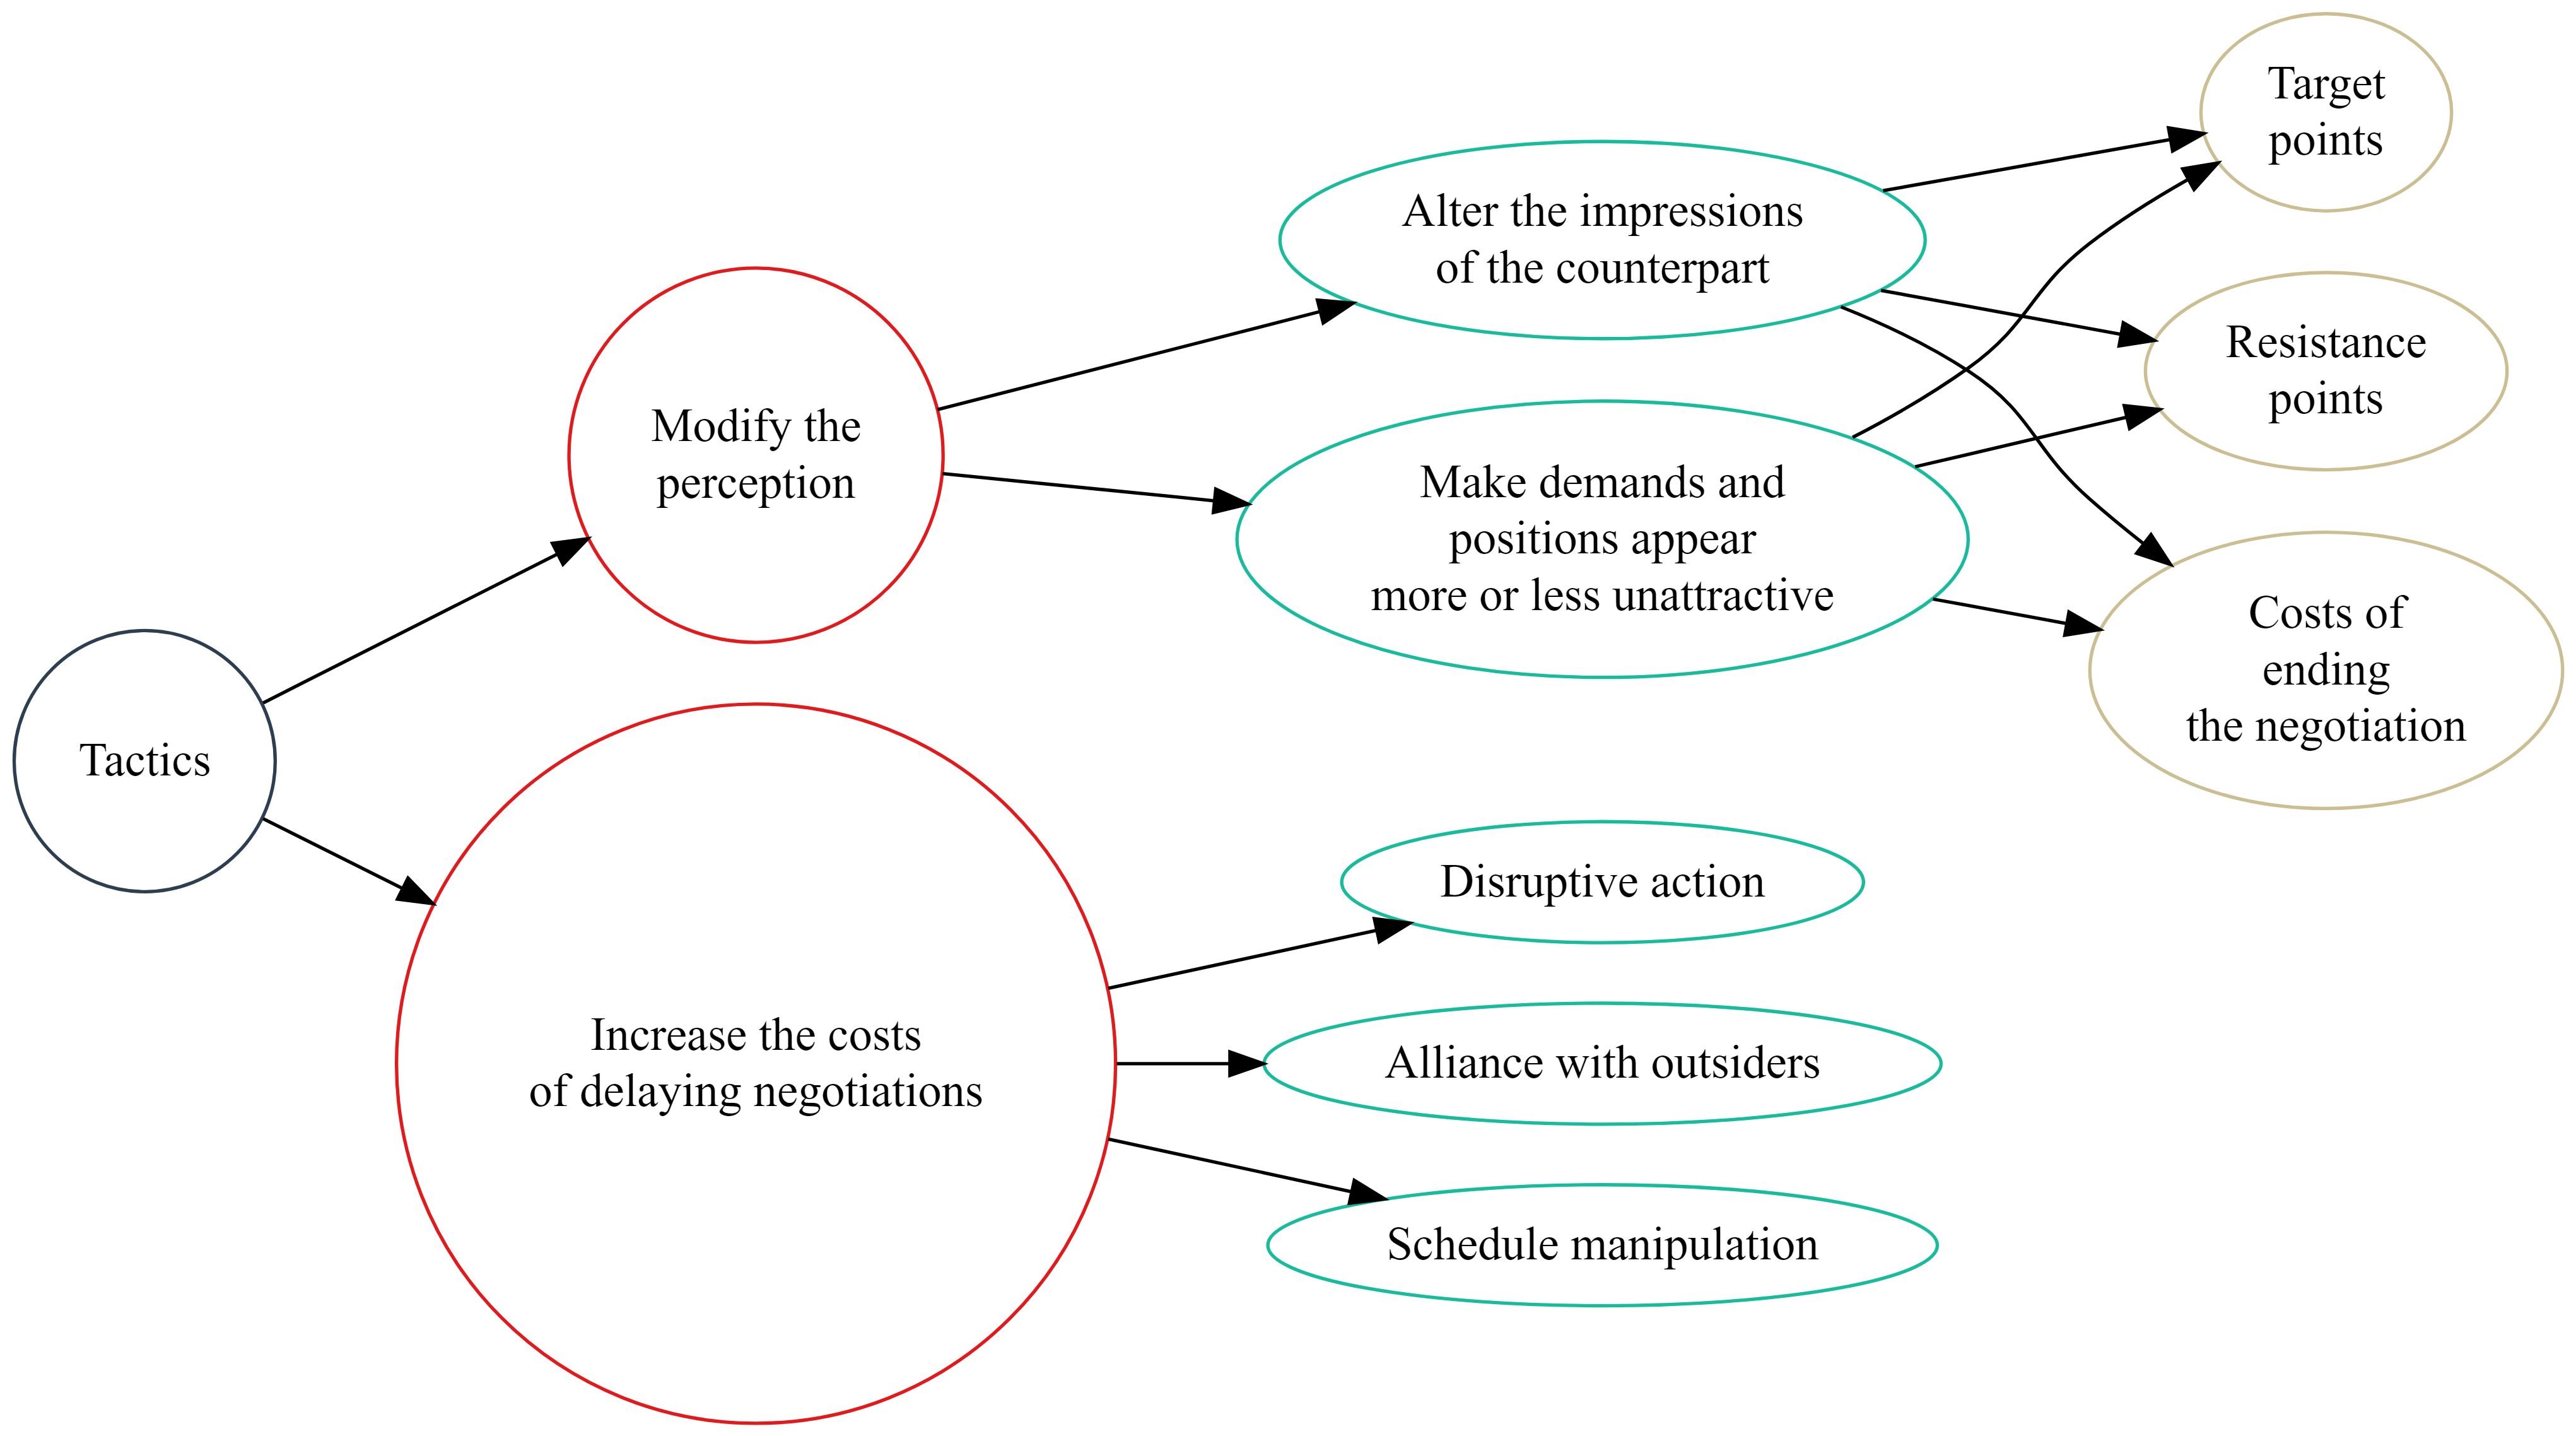
\includegraphics[width=4.5in,height=2.5in]{002_stra_tac_distri_files/figure-beamer/dot-figure-4.png}

}

\caption{\label{fig-tactics-distributive-bargaining-2}Tactics
distributive bargaining
(\citeproc{ref-lewicki_negociacion_2024}{Lewicki, Barry, and Saunders
2024, 42--48})}

\end{figure}%
\end{frame}

\section{Aspects about taking positions during a
negotiation}\label{aspects-about-taking-positions-during-a-negotiation}

\begin{frame}{}
\phantomsection\label{section-12}
\begin{itemize}
\item
  In (\citeproc{ref-lewicki_negociacion_2024}{Lewicki, Barry, and
  Saunders 2024, chap. 2}, p 48-55) the recommended positions to be
  taken with regard to the following elements are pointed out:

  \begin{itemize}
  \item
    \textbf{Opening offers}

    \begin{itemize}
    \tightlist
    \item
      Who should make the first offer?
    \item
      What should be the initial offer?
    \item
      Should the offer be perceived as low, moderate or high by the
      other party?
    \item
      Should the initial offer be near or far from our own resistance
      point?
    \end{itemize}
  \item
    \textbf{Opening stance}

    \begin{itemize}
    \tightlist
    \item
      Should a moderate or aggressive stance be taken?
    \end{itemize}
  \item
    \textbf{Initial concessions}

    \begin{itemize}
    \tightlist
    \item
      How wide should the initial concession be?
    \end{itemize}
  \item
    \textbf{Final offer}

    \begin{itemize}
    \tightlist
    \item
      How to communicate that a particular offer is a final offer?
    \end{itemize}
  \end{itemize}
\end{itemize}
\end{frame}

\section{Commitments}\label{commitments}

\begin{frame}{}
\phantomsection\label{section-13}
\begin{itemize}
\item
  \textbf{Commitment} means taking a stance in a negotiation and making
  a explicit or implicit promise about future actions.

  \begin{itemize}
  \item
    A commitment is a way to create a bargaining position by specifying
    a future action if a position is not reached.
  \item
    A commitment aims to clarify the negotiator's planned actions and
    eliminate any uncertainty about their intentions.

    \begin{itemize}
    \item
      However, they may also fix a negotiator to a particular position
      (\citeproc{ref-lewicki_negociacion_2024}{Lewicki, Barry, and
      Saunders 2024, chap. 2}, p 56)
    \item
      That is why when making commitments, one should also make
      contingency plans for a graceful exit if needed
    \item
      Also it is important to point out that good, sound and deliberate
      commitments take time to establish so it is important to don't
      commit prematurely
      (\citeproc{ref-lewicki_negociacion_2024}{Lewicki, Barry, and
      Saunders 2024, chap. 2}, p 56)
    \end{itemize}
  \end{itemize}
\end{itemize}
\end{frame}

\begin{frame}{}
\phantomsection\label{section-14}
\begin{figure}

\centering{

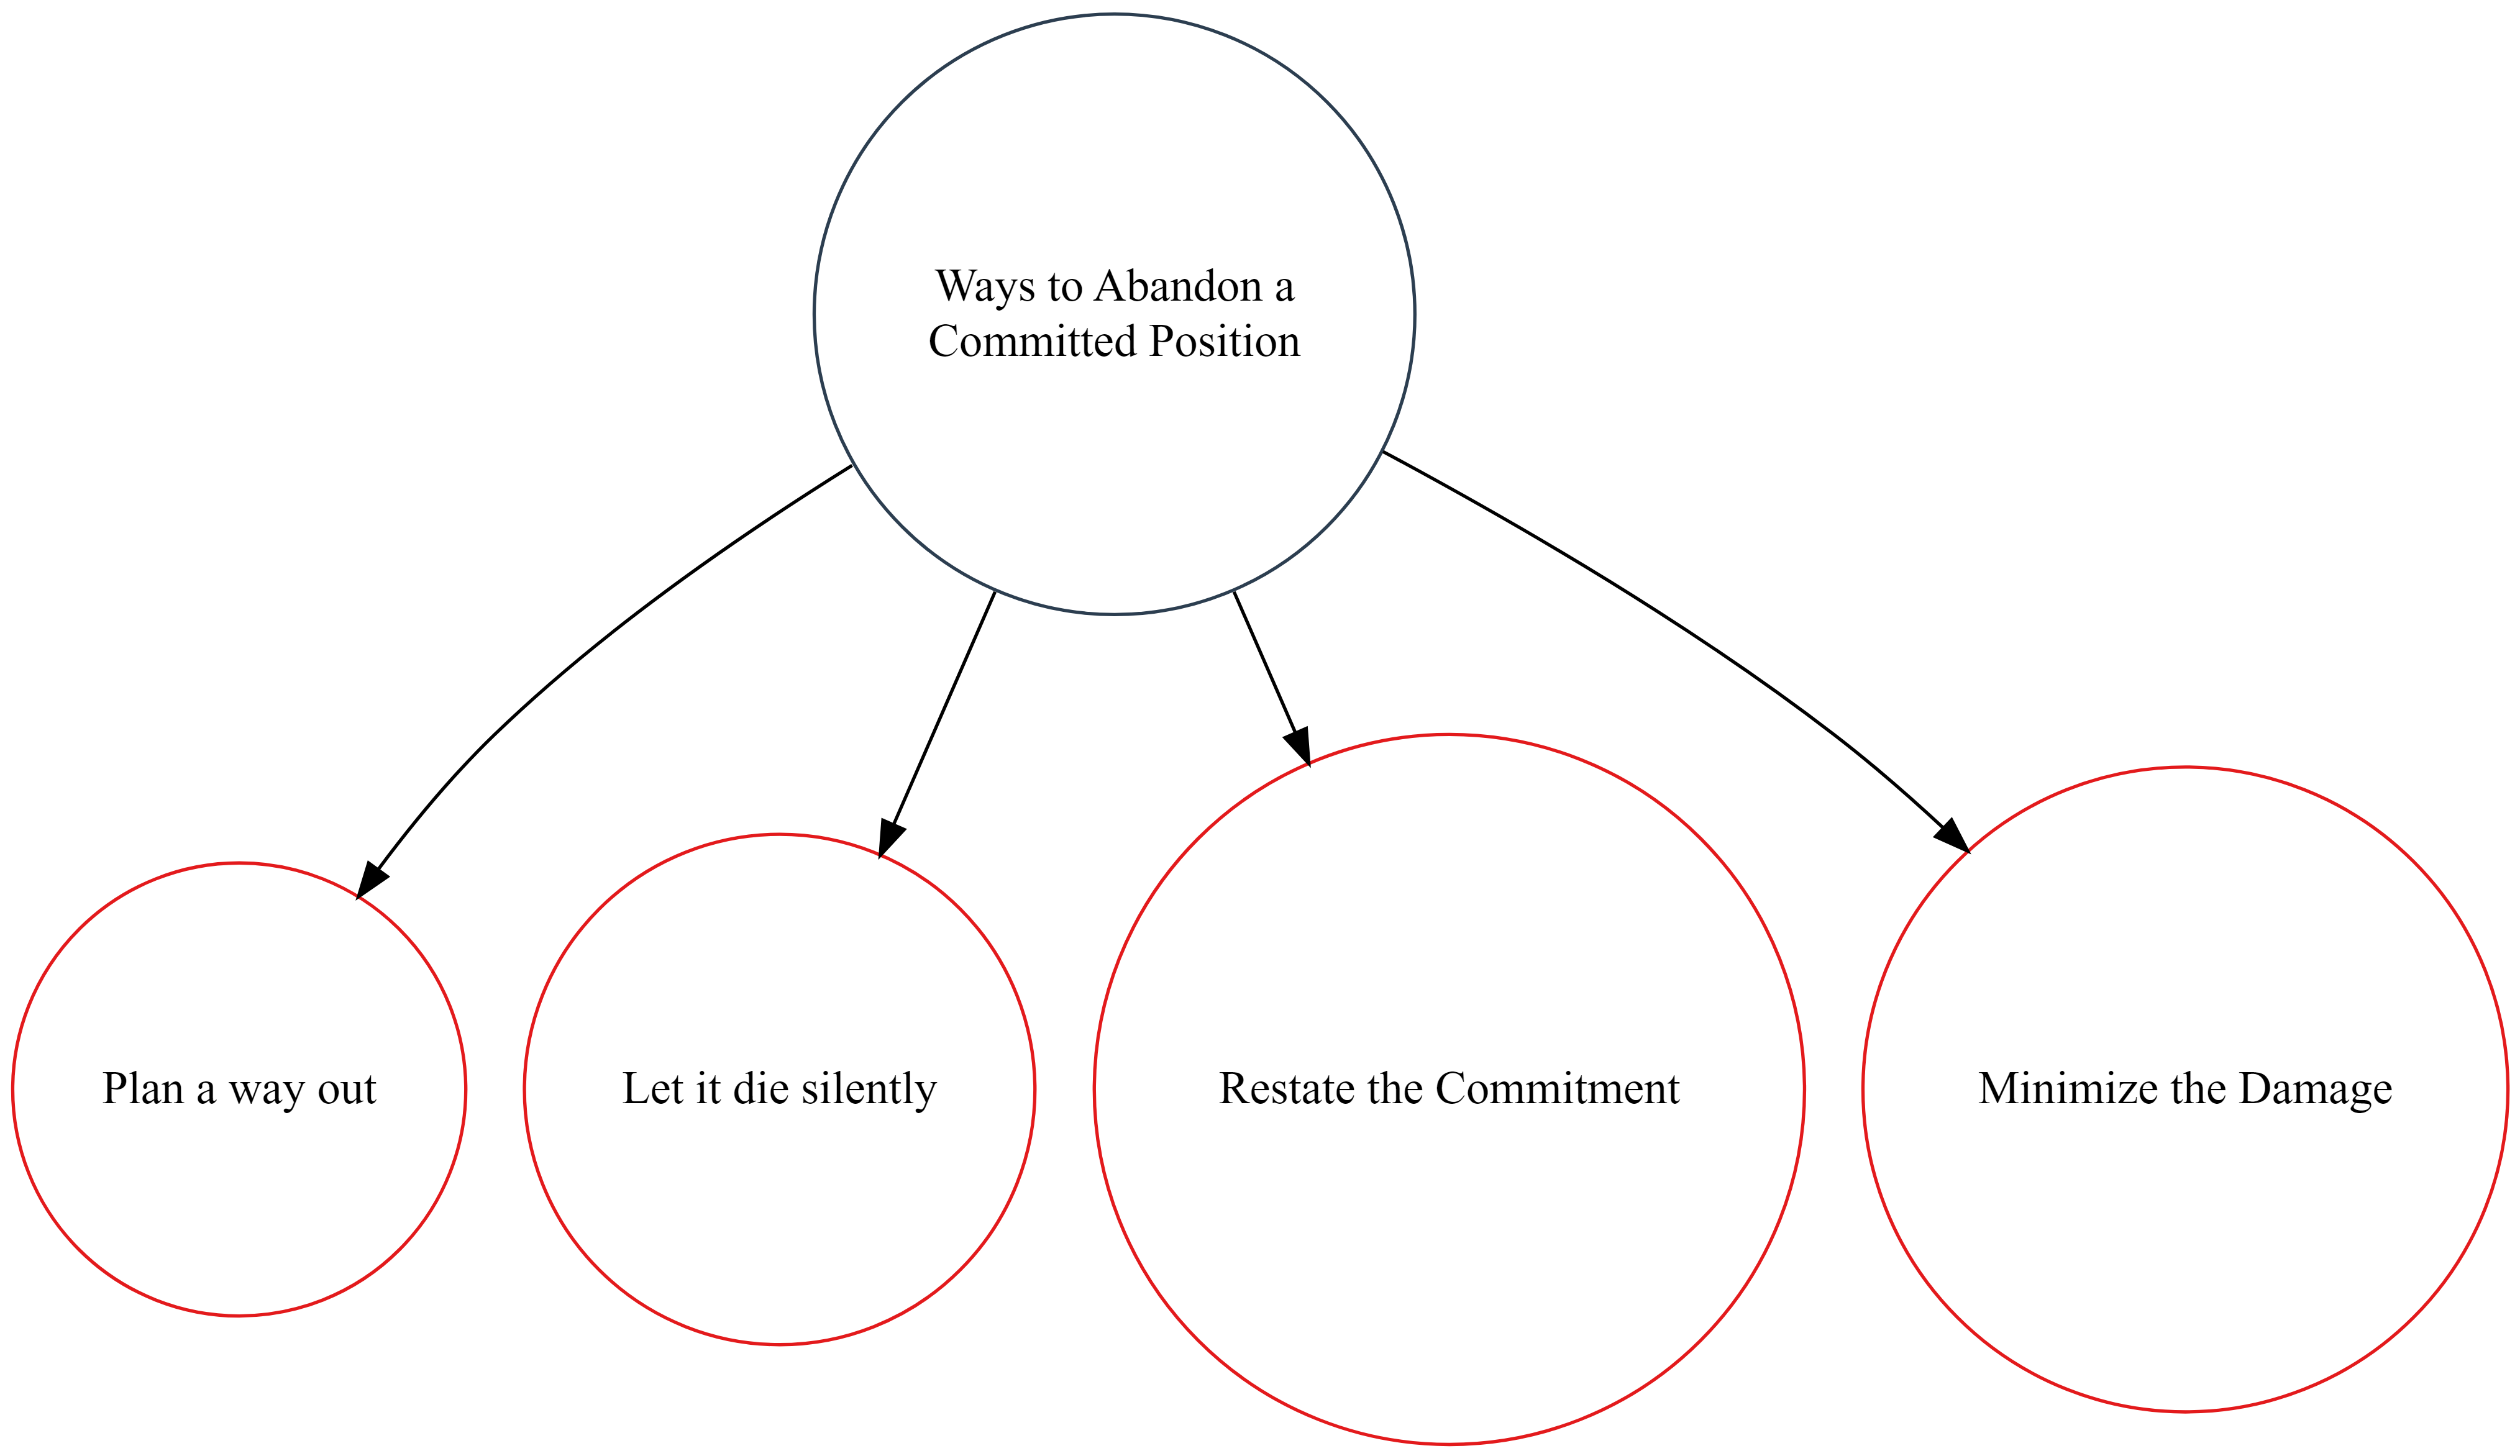
\includegraphics[width=4.5in,height=2.5in]{002_stra_tac_distri_files/figure-beamer/dot-figure-3.png}

}

\caption{\label{fig-ways-to-abandon-committed-position}Ways to abandon a
committed position (\citeproc{ref-lewicki_negociacion_2024}{Lewicki,
Barry, and Saunders 2024, 58--59})}

\end{figure}%
\end{frame}

\section{Closing a deal}\label{closing-a-deal}

\begin{frame}{}
\phantomsection\label{section-15}
\begin{itemize}
\item
  The negotiations seek to reach an agreement if
  possible\footnote<.->{Remember that negotiation as a form of decision
    making is not the only method that exists!}. In order to achieve
  that goal with a greater probability, the following practices are
  recommended based on what is pointed out in
  (\citeproc{ref-lewicki_negociacion_2024}{Lewicki, Barry, and Saunders
  2024, chap. 2}, p 59-60):

  \begin{itemize}
  \item
    Offer similar options to the other parties to make the negotiation
    more flexible.
  \item
    Assume a closing technique or stance.
  \item
    Split the difference when a \textbf{mutual adjustment} process has
    been carried out.
  \item
    Use \textbf{exploding offers} that refers to setting a deadline
    where a specific proposal is in force for a limited time.
  \item
    Use \textbf{sweeteners} that refers to granting special concessions
    before closing.
  \end{itemize}
\end{itemize}
\end{frame}

\section{How to face hardball
tactics?}\label{how-to-face-hardball-tactics}

\begin{frame}{}
\phantomsection\label{section-16}
\begin{itemize}
\item
  Sometimes in negotiations people use \textbf{hardball tactics}. In
  general in (\citeproc{ref-lewicki_negociacion_2024}{Lewicki, Barry,
  and Saunders 2024, chap. 2}, p 61) the authors recommend not to use
  them as they cause damage in the negotiation process. However, it is
  important to know them and know how to deal with them.
\item
  In (\citeproc{ref-lewicki_negociacion_2024}{Lewicki, Barry, and
  Saunders 2024, chap. 2}, pp 61-62) 4 possible strategies to face these
  tactics are pointed out:

  \begin{itemize}
  \tightlist
  \item
    Discuss them
  \item
    Ignore them
  \item
    Respond in kind
  \item
    Co-opt the other party
  \end{itemize}
\end{itemize}
\end{frame}

\begin{frame}{}
\phantomsection\label{section-17}
\begin{figure}

\centering{

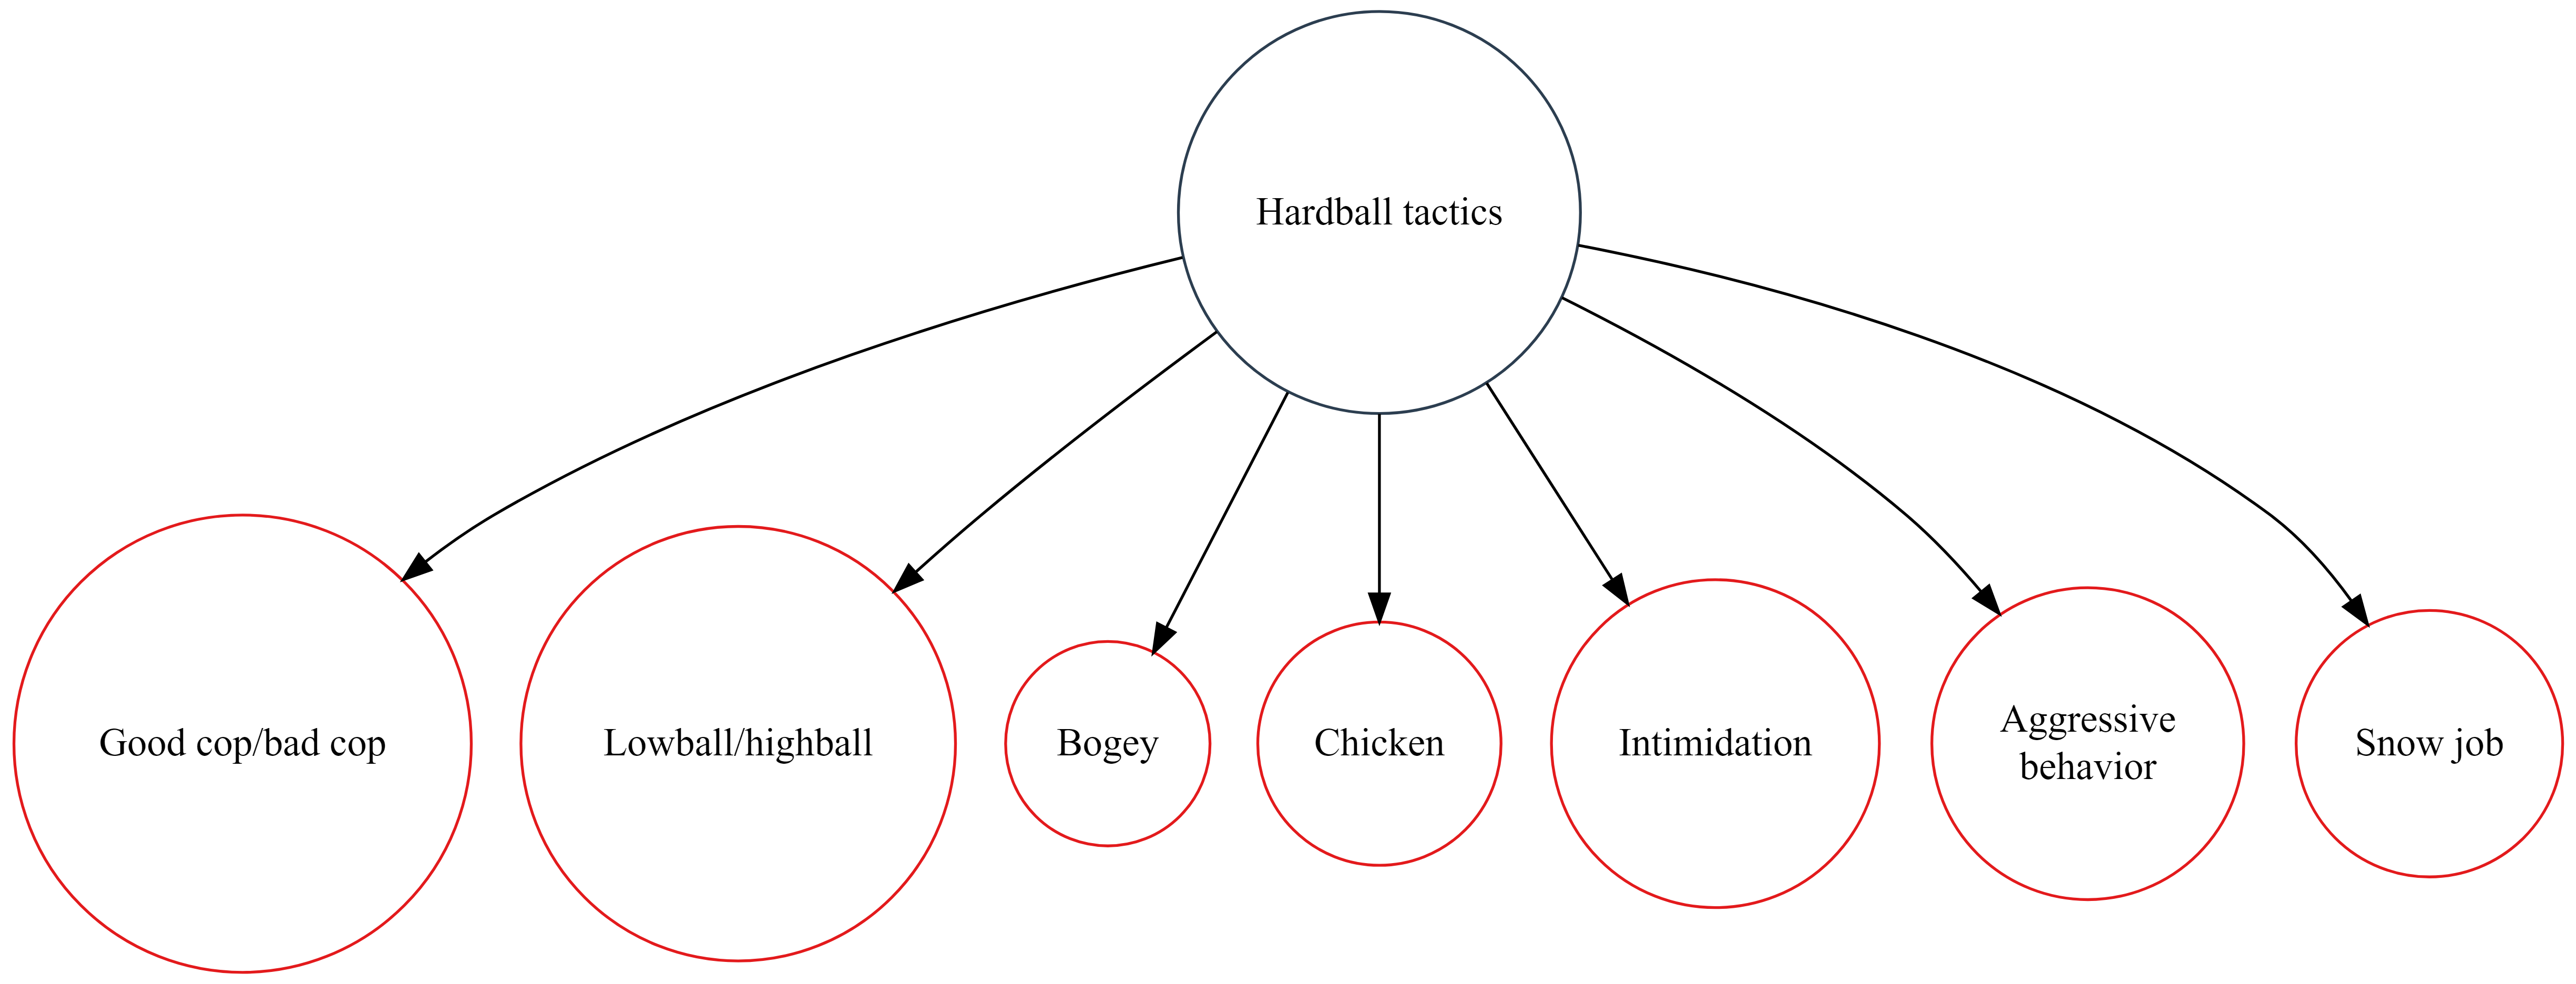
\includegraphics[width=4.5in,height=2.5in]{002_stra_tac_distri_files/figure-beamer/dot-figure-2.png}

}

\caption{\label{fig-hard-ball-tactics}Typical hardball tactics
(\citeproc{ref-lewicki_negociacion_2024}{Lewicki, Barry, and Saunders
2024}, p 63)}

\end{figure}%
\end{frame}

\section{Acknowledgments}\label{acknowledgments}

\begin{frame}{}
\phantomsection\label{section-18}
\begin{itemize}
\item
  To my family that supports me
\item
  To the taxpayers of Colombia and the
  \href{https://www.umng.edu.co/estudiante}{\textbf{UMNG students}} who
  pay my salary
\item
  To the \href{https://www.business-science.io/}{\textbf{Business
  Science}} and \href{https://www.rfordatasci.com/}{\textbf{R4DS Online
  Learning}} communities where I learn
  \href{https://www.r-project.org/about.html}{\textbf{R}} and
  \href{https://www.python.org/about/}{\textbf{\(\pi\)-thon}}
\item
  To the \href{https://www.r-project.org/contributors.html}{\textbf{R
  Core Team}}, the creators of
  \href{https://rstudio.com/products/rstudio/}{\textbf{RStudio IDE}},
  \href{https://quarto.org/}{\textbf{Quarto}} and the authors and
  maintainers of the packages
  \href{https://CRAN.R-project.org/package=tidyverse}{\textbf{tidyverse}},
  \href{https://CRAN.R-project.org/package=tidyquant}{\textbf{tidyquant}},
  \href{https://CRAN.R-project.org/package=ggrepel}{\textbf{ggrepel}},
  \href{https://CRAN.R-project.org/package=DiagrammeR}{\textbf{DiagrammeR}}
  and
  \href{https://CRAN.R-project.org/package=tinytex}{\textbf{tinytex}}
  for allowing me to access these tools without paying for a license
\item
  To the \href{https://www.kernel.org/category/about.html}{\textbf{Linux
  kernel community}} for allowing me the possibility to use some
  \href{https://static.lwn.net/Distributions/}{\textbf{Linux
  distributions}} as my main
  \href{https://en.wikipedia.org/wiki/Operating_system}{\textbf{OS}}
  without paying for a license
\end{itemize}
\end{frame}

\section*{References}\label{references}
\addcontentsline{toc}{section}{References}

\begin{frame}[allowframebreaks]{References}
\phantomsection\label{refs}
\begin{CSLReferences}{1}{0}
\bibitem[\citeproctext]{ref-lewicki_negociacion_2024}
Lewicki, Roy J., Bruce Barry, and David M. Saunders. 2024.
\emph{Negociación}. 9th ed. McGraw-Hill Education.
\url{https://www-ebooks7-24-com.ezproxy.umng.edu.co/?il=40562}.

\bibitem[\citeproctext]{ref-muthoo_bargaining_1999}
Muthoo, Abhinay. 1999. \emph{Bargaining Theory with Applications}. New
York: Cambridge University Press.

\end{CSLReferences}
\end{frame}




\end{document}
